\chapter{Research Methodology}

This chapter outlines the methodology employed in developing AlgoBugs, a diagnostic benchmark for evaluating Large Language Models on targeted fault exposure tasks. The methodology covers design specifications, data collection procedures, and evaluation protocols for reliable assessment of LLM reasoning capabilities.

\section{Methodology/Requirement Analysis \& Design Specification}
\subsection{Overview}

The development of AlgoBugs follows a structured methodology that addresses the limitations of existing benchmarks through bug taxonomy design, careful data curation, and execution-based evaluation protocols.

The methodology proceeds in stages: first, an eight-category bug taxonomy is established through analysis of competitive programming failure modes. This is followed by data collection from recent Codeforces submissions to ensure temporal freshness and reduce contamination risk. Each problem-bug pair is then validated through automated differential testing and expert review.

The evaluation protocol focuses on diagnostic assessment rather than simple accuracy metrics, enabling analysis of model capabilities across specific categories of algorithmic reasoning.

\subsection{Proposed Methodology/ System Design}

The AlgoBugs development process follows a defined workflow designed to ensure high-quality benchmark construction and reliable evaluation results. Figure \ref{fig:methodology} illustrates the complete methodology flowchart, showing the progression from initial data collection through final diagnostic evaluation.

\begin{figure}[h!]
\centering
\begin{tikzpicture}[
    node distance=0.55cm and 2.5cm,
    box/.style={rectangle, rounded corners=3pt, draw=black!70, fill=blue!8,
                text width=5.8cm, align=center, font=\small, minimum height=0.65cm, inner sep=4pt},
    highlight/.style={rectangle, rounded corners=3pt, draw=black, fill=gray!20,
                text width=5.8cm, align=center, font=\small\bfseries, minimum height=0.65cm, inner sep=4pt},
    arr/.style={->, >=Stealth, thick, draw=black!60}
]
\node[highlight] (cf)      {Codeforces Platform\\{\footnotesize WA $\rightarrow$ AC submission histories}};
\node[box, below=of cf]    (ext)     {Custom Chrome Extension\\{\footnotesize Automated WA/AC pair extraction per problem}};
\node[box, below=of ext]   (review)  {Manual Review \& Quality Filtering\\{\footnotesize Diff analysis · subtlety verification · noise removal}};
\node[box, below=of review](label)   {Expert Taxonomy Labelling\\{\footnotesize Each pair assigned T1--T8 · IRR validated}};
\node[highlight, below=of label] (ds) {AlgoBugs Dataset\\{\footnotesize 1{,}000 pairs · 40 problems · 8 difficulty brackets}};
\node[box, below=of ds]    (api)     {LLM API (OpenRouter)\\{\footnotesize 5 models $\times$ 3 prompt strategies = 15 experiments}};
\node[box, below=of api]   (parse)   {Test Case Extraction\\{\footnotesize \texttt{<test>} tag parser with 3-level fallback}};
\node[box, below=of parse] (diff)    {Differential Testing Engine\\{\footnotesize g++ C++20 compile \& execute · output comparison}};
\node[highlight, below=of diff] (out) {\textsc{BUG\_EXPOSED} / \textsc{NOT\_EXPOSED} / Excluded\\{\footnotesize Per-pair verdict with full execution log}};
\node[box, below=of out]   (fer)     {FER Calculation\\{\footnotesize Per model · per bug category · per prompting strategy}};

\draw[arr] (cf)     -- (ext);
\draw[arr] (ext)    -- (review);
\draw[arr] (review) -- (label);
\draw[arr] (label)  -- (ds);
\draw[arr] (ds)     -- (api);
\draw[arr] (api)    -- (parse);
\draw[arr] (parse)  -- (diff);
\draw[arr] (diff)   -- (out);
\draw[arr] (out)    -- (fer);
\end{tikzpicture}
\caption{End-to-end AlgoBugs pipeline: from Codeforces data collection through execution-based differential testing to per-category Fault Exposure Rate computation.}
\label{fig:methodology}
\end{figure}

The systematic workflow includes the following key stages:

\begin{enumerate}
    \item \textbf{Bug Taxonomy Development:} Analysis of competitive programming solutions and their failure modes to establish an eight-category classification of algorithmic bugs across domains (dynamic programming, greedy algorithms, graph algorithms, etc.).
    
    \item \textbf{Problem Selection:} Careful selection of competitive programming problems from Codeforces based on criteria including problem diversity, difficulty distribution, and temporal freshness to mitigate data contamination concerns.
    
    \item \textbf{Bug Pair Mining:} Automated extraction of \{Wrong Answer, Accepted\} submission pairs from recent Codeforces contests, focusing on submissions that differ minimally to isolate specific bug types.
    
    \item \textbf{Quality Validation:} Multi-stage validation process involving automated testing of bug reproducibility, expert review of bug authenticity, and verification of diagnostic value for each problem-bug pair.
    
    \item \textbf{Benchmark Construction:} Systematic organization of validated problem-bug pairs according to the established taxonomy, ensuring balanced representation across different bug categories and difficulty levels.
    
    \item \textbf{Evaluation Protocol:} Implementation of an execution-based evaluation method that measures both overall FER and per-category performance to support diagnostic analysis.

    \item \textbf{Statistical Analysis:} Application of inter-rater reliability (Cohen's Kappa) and per-category FER aggregation to identify performance patterns and limitations across model tiers.
\end{enumerate}

\subsubsection{Resource and Performance Failures}

\begin{itemize}
    \item \textbf{Time Limit Exceeded (TLE):} This includes not only naive complexity bugs but also high-constant-factor solutions that fail on maximum-sized inputs, or algorithms that are vulnerable to worst-case inputs (e.g., a long chain in a graph traversal). This is a known weakness for LLMs \cite{wang2025robustness, cao2025tcgbench}.
    
    \item \textbf{Memory Limit Exceeded (MLE):} Bugs that are exposed by inputs forcing the creation of unexpectedly large data structures. These failures often result from poor space complexity analysis or inefficient data structure choices.
\end{itemize}

\subsubsection{Boundary, Edge Case, and Data Type Errors}

\begin{itemize}
    \item \textbf{Numeric Boundary/Overflow:} Errors related to minimum/maximum constraint values, zero, or intermediate calculations exceeding the capacity of standard data types (e.g., int vs. long long). These represent fundamental programming errors that are common in competitive programming.
    
    \item \textbf{Structural Edge Cases:} Errors exposed by empty inputs, single-element collections, or inputs where all elements are identical \cite{wang2025robustness}. These bugs reveal insufficient consideration of boundary conditions in algorithm design.
\end{itemize}

\subsection{Data Sourcing and Curation Protocol}

AlgoBugs is built from real bugs mined directly from Codeforces submissions. Using real submissions rather than synthetic mutations means the bugs reflect genuine human errors and the fixes reflect genuine human corrections \cite{huang2024competition, haque2023fixeval}.

\textbf{Technical data collection challenge.} Codeforces does not expose submission source code through its public API. Direct HTTP scraping is blocked by Cloudflare's bot-detection layer. Two alternatives were evaluated: manual copy-paste (infeasible for 1,000 pairs across 40 problems) and a custom Chrome extension running inside an authenticated browser session (viable, because the extension operates within a real browser context that passes Cloudflare's human-verification checks). The extension was chosen and built specifically for this project. It implements deliberate rate limiting to respect Codeforces infrastructure: a configurable inter-request delay (default 3 seconds), a burst limit of 8 requests before a mandatory 15-second cooldown, and a practical ceiling of 25 pairs collected per session. Figure~\ref{fig:ext_architecture} shows the three-layer architecture of the extension.

\begin{figure}[h!]
\centering
\pgfdeclarelayer{bg}
\pgfsetlayers{bg,main}
\begin{tikzpicture}[
    node distance=0.45cm and 2.4cm,
    box/.style={rectangle, rounded corners=3pt, draw=black!65, fill=blue!8,
                text width=4.8cm, align=center, font=\small,
                minimum height=0.9cm, inner sep=5pt},
    ext/.style={rectangle, rounded corners=4pt, draw=black!55, fill=gray!10,
                text width=3.0cm, align=center, font=\small,
                minimum height=1.1cm, inner sep=6pt},
    arr/.style={->, >=Stealth, thick, draw=black!55}
]
\node[box] (ui)     {Popup Interface\\{\footnotesize Problem ID \textbullet{} Pair count \textbullet{} Language filter}};
\node[box, below=of ui]     (engine) {Request Engine\\{\footnotesize Rate-limited queue \textbullet{} Burst/cooldown \textbullet{} Retry}};
\node[box, below=of engine] (zip)    {ZIP Packager\\{\footnotesize metadata.json \textbullet{} source code \textbullet{} problem statement}};

\begin{pgfonlayer}{bg}
    \node[rectangle, draw=black!35, dashed, rounded corners=5pt, fill=blue!3,
          inner sep=10pt, fit=(ui)(engine)(zip),
          label={[font=\small\bfseries]above:Chrome Extension (Manifest V3)}] {};
\end{pgfonlayer}

\node[ext, left=2.2cm of engine]  (cf) {Codeforces\\{\footnotesize HTTPS via browser\\\footnotesize (Cloudflare-safe)}};
\node[ext, right=2.2cm of engine] (ds) {AlgoBugs\\Dataset\\{\footnotesize ZIP archives\\\footnotesize downloaded locally}};

\draw[arr] (ui)     -- node[right, font=\scriptsize]{config} (engine);
\draw[arr] (engine) -- node[right, font=\scriptsize]{pair data} (zip);
\draw[arr] (cf)     -- node[above, font=\scriptsize, sloped]{submission code} (engine);
\draw[arr] (zip)    -- node[above, font=\scriptsize, sloped]{pair ZIPs} (ds);
\end{tikzpicture}
\caption{Architecture of the Codeforces Submission Extractor Chrome extension. The popup interface accepts researcher configuration; the request engine fetches submission code from Codeforces through rate-limited HTTPS calls that pass Cloudflare bot-detection; the ZIP packager assembles each WA/AC pair into the standard AlgoBugs format for download.}
\label{fig:ext_architecture}
\end{figure}

The curation protocol for each data point follows these steps:

\begin{enumerate}
    \item \textbf{Problem Selection:} Problems are selected from recent Codeforces contests held after the knowledge cutoff dates of the LLMs being evaluated, to minimize data contamination \cite{huang2024competition}.
    
    \item \textbf{Pair Mining:} We identify submission pairs from the same user for the same problem, consisting of a "Wrong Answer" (or TLE/MLE) submission followed by an "Accepted" submission. This ensures that we capture real debugging scenarios.
    
    \item \textbf{Bug Isolation:} The two submissions are compared using a diff utility. Only pairs with small, localized changes are kept to ensure the bug is isolated and the fix is minimal. This prevents the inclusion of major algorithmic rewrites.
    
    \item \textbf{Subtlety Verification:} The buggy solution is compiled and run against the public sample test cases provided in the problem description. The data point is only accepted if the buggy solution passes all public sample tests. This is a critical quality gate to ensure the bug is a true corner case and not a trivial error.
    
    \item \textbf{Taxonomy Classification:} The isolated bug is manually analyzed and classified according to the taxonomy defined above. This classification is performed by experienced competitive programmers to ensure accuracy.
\end{enumerate}

\subsection{Dataset Structure}

Each curated data point is stored in a structured, machine-readable format to ensure reproducibility and ease of use. The dataset organization includes:

\begin{itemize}
    \item A master \texttt{metadata.json} file that indexes each problem, its buggy variants, the bug category, and a natural language description of the bug.
    \item Individual directories for each problem containing:
    \begin{itemize}
        \item \texttt{problem\_statement.md}: The complete problem description
        \item \texttt{solution\_correct.cpp}: The accepted solution
        \item \texttt{solution\_buggy.cpp}: The buggy solution
        \item \texttt{test\_cases/}: Directory containing sample test cases
    \end{itemize}
\end{itemize}

This organization ensures clarity, reproducibility, and ease of integration with evaluation frameworks.

Figure~\ref{fig:rating_dist} shows the distribution across difficulty brackets. Each of the eight rating levels contributes exactly 125 pairs, producing a perfectly balanced benchmark across difficulty.

\begin{figure}[h!]
\centering
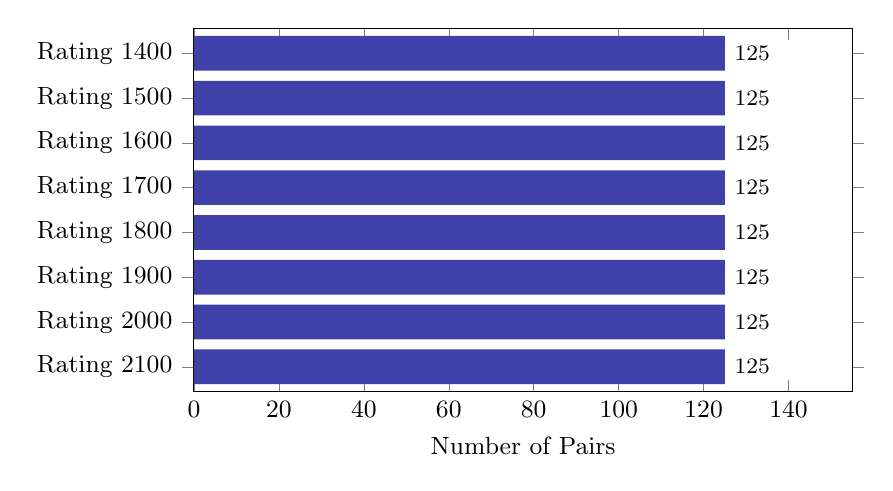
\begin{tikzpicture}
\begin{axis}[
    xbar,
    width=0.82\linewidth,
    height=6.2cm,
    xlabel={Number of Pairs},
    symbolic y coords={2100,2000,1900,1800,1700,1600,1500,1400},
    ytick=data,
    yticklabels={Rating 2100, Rating 2000, Rating 1900, Rating 1800, Rating 1700, Rating 1600, Rating 1500, Rating 1400},
    nodes near coords,
    nodes near coords style={font=\footnotesize},
    nodes near coords align={horizontal},
    xmin=0, xmax=155,
    bar width=0.44cm,
    enlarge y limits=0.08,
    tick label style={font=\small},
    label style={font=\small},
]
\addplot[fill=blue!55!black!75, draw=none] coordinates {
    (125,2100)(125,2000)(125,1900)(125,1800)
    (125,1700)(125,1600)(125,1500)(125,1400)
};
\end{axis}
\end{tikzpicture}
\caption{Uniform distribution of the 1,000 AlgoBugs pairs across eight Codeforces difficulty rating brackets (1400--2100). Each bracket contains five problems with 25 pairs each.}
\label{fig:rating_dist}
\end{figure}

\subsection{Bug Taxonomy (T1--T8)}

The taxonomy is the central intellectual contribution of this work. Figure~\ref{fig:taxonomy} illustrates the three-tier, eight-category hierarchy. The number of categories was chosen to balance diagnostic resolution (more categories reveal finer distinctions) against statistical depth (fewer categories yield more samples per class for robust analysis). Eight categories produces approximately 125 samples per class across the 1,000-pair dataset, providing sufficient statistical power for per-category analysis.

\begin{figure}[h!]
\centering
\begin{tikzpicture}[
    root/.style={rectangle, rounded corners=4pt, draw=black, fill=gray!25,
                 text width=4.6cm, align=center, font=\bfseries\small, minimum height=0.75cm},
    tier/.style={rectangle, rounded corners=3pt, draw=black!70, fill=blue!12,
                 text width=3.2cm, align=center, font=\small\bfseries, minimum height=0.65cm},
    leaf/.style={rectangle, rounded corners=2pt, draw=black!50, fill=blue!8,
                 text width=1.42cm, align=center, font=\scriptsize, minimum height=0.75cm},
    arr/.style={->, >=Stealth, draw=black!50}
]
% 8 leaf nodes placed at equal 1.72cm spacing
\node[leaf] (L1) at (0.00cm,-3.6cm) {\textbf{T1}\\Integer\\Overflow};
\node[leaf] (L2) at (1.72cm,-3.6cm) {\textbf{T2}\\Modular\\Arith.};
\node[leaf] (L3) at (3.44cm,-3.6cm) {\textbf{T3}\\Off-by-\\One};
\node[leaf] (L4) at (5.16cm,-3.6cm) {\textbf{T4}\\Wrong\\Cond.};
\node[leaf] (L5) at (6.88cm,-3.6cm) {\textbf{T5}\\Algo.\\Flaw};
\node[leaf] (L6) at (8.60cm,-3.6cm) {\textbf{T6}\\State/\\Init};
\node[leaf] (L7) at (10.32cm,-3.6cm) {\textbf{T7}\\Corner\\Case};
\node[leaf] (L8) at (12.04cm,-3.6cm) {\textbf{T8}\\I/O\\Format};
% Tier nodes centered over their leaf groups
\node[tier] (T1) at (0.86cm,-1.8cm)  {Tier 1\\Data \& Type};
\node[tier] (T2) at (5.16cm,-1.8cm)  {Tier 2\\Control \& Logic};
\node[tier] (T3) at (10.32cm,-1.8cm) {Tier 3\\State \& Edge};
% Root centered over all tiers
\node[root] (root) at (5.59cm,0cm) {AlgoBugs Taxonomy\\8 Bug Categories};
% Edges root → tiers
\draw[arr] (root) -- (T1);
\draw[arr] (root) -- (T2);
\draw[arr] (root) -- (T3);
% Edges tiers → leaves
\draw[arr] (T1) -- (L1);  \draw[arr] (T1) -- (L2);
\draw[arr] (T2) -- (L3);  \draw[arr] (T2) -- (L4);  \draw[arr] (T2) -- (L5);
\draw[arr] (T3) -- (L6);  \draw[arr] (T3) -- (L7);  \draw[arr] (T3) -- (L8);
\end{tikzpicture}
\caption{The AlgoBugs three-tier, eight-category bug taxonomy. Each leaf node represents a qualitatively distinct class of algorithmic error requiring a different form of LLM reasoning to expose.}
\label{fig:taxonomy}
\end{figure}

Table~\ref{tab:taxonomy_detail} provides the formal definition of each category including its technical signature and the final distribution in the AlgoBugs dataset.

\begin{table}[h!]
\centering
\caption{AlgoBugs taxonomy: category definitions and dataset distribution.}
\label{tab:taxonomy_detail}
\renewcommand{\arraystretch}{1.25}
\begin{tabular}{clp{6.5cm}r}
\toprule
\textbf{ID} & \textbf{Category} & \textbf{Technical Signature} & \textbf{Count} \\
\midrule
T1 & Integer Overflow    & Using \texttt{int} where \texttt{long long} is required; silent wrap-around on operations exceeding $2\times10^9$ & 66 \\
T2 & Modular Arithmetic  & Missing \texttt{\% MOD} at intermediate steps; negative subtraction without \texttt{+MOD} guard & 39 \\
T3 & Off-by-One          & Loop bound errors (\texttt{< n} vs \texttt{<= n}); fence-post errors; 0-vs-1 index mismatches & 137 \\
T4 & Wrong Conditional   & Inverted branch logic; wrong relational operator (\texttt{>} vs \texttt{>=}); \texttt{\&\&}/\texttt{||} confusion & 308 \\
T5 & Algorithmic Flaw    & Logic passes sample tests but fails globally; incorrect greedy choice; missing DP state & 274 \\
T6 & State / Init        & Failing to reset global arrays or visited sets between test cases in multi-case problems & 80 \\
T7 & Corner Case         & Sound general logic but crashes/fails on $N{=}0$, $N{=}1$, empty input, or max constraints & 47 \\
T8 & I/O Format          & Wrong variable read order; extra whitespace; missing newline; incorrect output format & 49 \\
\midrule
\multicolumn{3}{r}{\textbf{Total}} & \textbf{1,000} \\
\bottomrule
\end{tabular}
\end{table}

Figure~\ref{fig:taxonomy_dist} shows the distribution of pairs across the eight categories. T4 (Wrong Conditional) and T5 (Algorithmic Flaw) are the most frequent, together accounting for 58\% of the dataset, reflecting the dominance of logical and algorithmic reasoning failures in competitive programming. T1 (Integer Overflow) and T2 (Modular Arithmetic) are the least frequent, as these bugs require specific numerical conditions that are rarer in the general submission pool.

\begin{figure}[h!]
\centering
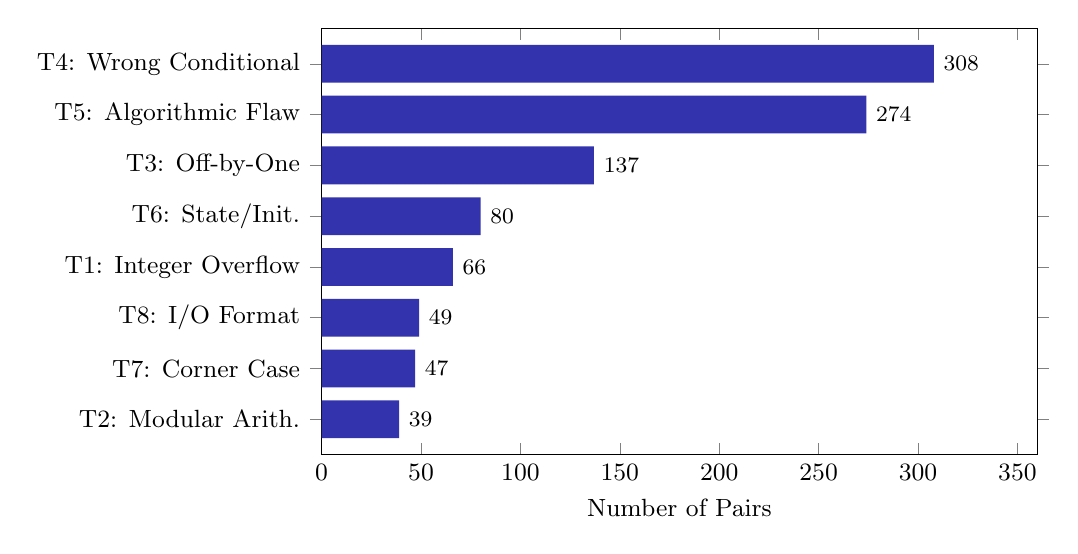
\begin{tikzpicture}
\begin{axis}[
    xbar,
    width=0.88\linewidth,
    height=7cm,
    xlabel={Number of Pairs},
    symbolic y coords={T2,T7,T8,T1,T6,T3,T5,T4},
    ytick=data,
    yticklabels={
        T2: Modular Arith.,
        T7: Corner Case,
        T8: I/O Format,
        T1: Integer Overflow,
        T6: State/Init.,
        T3: Off-by-One,
        T5: Algorithmic Flaw,
        T4: Wrong Conditional
    },
    nodes near coords,
    nodes near coords style={font=\footnotesize},
    nodes near coords align={horizontal},
    xmin=0, xmax=360,
    bar width=0.48cm,
    enlarge y limits=0.1,
    tick label style={font=\small},
    label style={font=\small},
]
\addplot[fill=blue!60!black!80, draw=none] coordinates {
    (39,T2)
    (47,T7)
    (49,T8)
    (66,T1)
    (80,T6)
    (137,T3)
    (274,T5)
    (308,T4)
};
\end{axis}
\end{tikzpicture}
\caption{Distribution of the 1,000 AlgoBugs pairs across the eight taxonomy categories, sorted by count. T4 (Wrong Conditional) and T5 (Algorithmic Flaw) together represent 58\% of all pairs.}
\label{fig:taxonomy_dist}
\end{figure}

\subsection{Experimental Setup}

The experimental design is crafted to evaluate an LLM's ability to perform targeted fault exposure, representing a more challenging and novel research frontier compared to general test suite generation \cite{yang2025testcase, cao2025tcgbench}.

\subsubsection{The Targeted Fault Exposure Task}

For each data point in the AlgoBugs benchmark, the LLM is provided with:

\begin{itemize}
    \item The complete problem description, including constraints and sample input/output
    \item The source code of a single buggy solution
    \item A request to generate a single test case input that causes the buggy solution to fail
\end{itemize}

The task requires the model to read the code, identify the logical flaw, and construct a specific input that triggers it. This is harder than general code understanding: the model must reason about what input values would push execution into the buggy branch or overflow the buggy variable.

\subsubsection{Prompt Engineering Strategies}

To understand the impact of different prompting approaches, the evaluation employs two prompting strategies:

\paragraph{Zero-Shot Prompting}

A baseline prompt that directly asks the LLM to generate a "hacking" test case without providing any examples \cite{dong2024survey}. This tests the model's inherent understanding of the task without additional context.

\textbf{Template:}
\begin{quote}
"Given the following competitive programming problem and a buggy solution, generate a single test case that will cause the buggy solution to fail while the correct solution would pass."
\end{quote}

\paragraph{Few-Shot Prompting}

Three synthetic worked examples are prepended to the prompt before the target pair \cite{promptpanda2025few, learnprompting2025shot}. Each example shows a short problem, a buggy C++ solution with the fault annotated in a comment, a brief analysis identifying why the bug triggers, and the exposing test input. The three examples cover one T1 (integer overflow from \texttt{int} multiplication), one T3 (off-by-one from a loop boundary stopping at index $n-2$), and one T4 (wrong comparison operator excluding equality). These categories were chosen to span the three most distinct reasoning patterns in the taxonomy.

The examples are synthetic, not drawn from the AlgoBugs dataset, to avoid data leakage. This design tests whether task-format demonstrations alone improve fault exposure, independent of category-specific grounding. A practical side effect: the worked examples anchor the \texttt{<test>} output format, producing zero \textsc{NO\_TEST\_GENERATED} failures across all 4,870 few-shot evaluations, compared to rates of 1--30\% under chain-of-thought prompting.

\paragraph{Chain-of-Thought Prompting}

The primary experimental prompt that explicitly instructs the LLM to first analyze the buggy code step-by-step to identify potential flaws, and then generate a test case based on that analysis. This technique is known to improve performance on complex reasoning tasks \cite{wei2022chain, li2025uncertainty}.

\textbf{Template:}
\begin{quote}
"Please analyze the given buggy code step by step:
1. Identify the main algorithm and approach
2. Look for potential logical errors, boundary issues, or performance problems
3. Based on your analysis, construct a test case that exploits the identified weakness"
\end{quote}

\begin{table}[h!]
\centering
\caption{Comparison of the three prompting strategies used in AlgoBugs.}
\label{tab:prompt_strategies}
\renewcommand{\arraystretch}{1.3}
\resizebox{\linewidth}{!}{%
\begin{tabular}{lp{3.8cm}p{3.2cm}p{4.5cm}}
\toprule
\textbf{Strategy} & \textbf{Model Input} & \textbf{Reasoning Mode} & \textbf{Key Property} \\
\midrule
Zero-Shot  & Problem statement + buggy code & Implicit & Baseline; no scaffolding or examples \\
Chain-of-Thought & Problem + buggy code + 3-step reasoning instruction & Explicit, structured & Forces step-by-step analysis before output \\
Few-Shot & Problem + buggy code + 3 synthetic worked examples & Example-guided & Demonstrates fault-targeting; anchors output format \\
\bottomrule
\end{tabular}%
}
\end{table}

\subsubsection{Model Selection and Configuration}

Five models spanning distinct capability tiers were selected for evaluation via the OpenRouter API:

\begin{itemize}
    \item \textbf{Gemini 2.0 Flash} (Google): mid-tier general model
    \item \textbf{DeepSeek V3} (DeepSeek): reasoning-oriented general model
    \item \textbf{LLaMA 3.3 70B Instruct} (Meta): open-source instruction-tuned model
    \item \textbf{Qwen3 Coder 30B} (Alibaba): code-specialist model
    \item \textbf{GPT-5.1} (OpenAI): frontier general model
\end{itemize}

All models were evaluated with temperature 1.0 and consistent generation parameters to ensure fair comparison across tiers.

\subsection{Evaluation Metrics}

The evaluation framework is designed to be objective and execution-based, which provides more reliable results than match-based metrics \cite{chen2021evaluating, haque2023fixeval}.

\subsubsection{Test Case Validity}

Before measuring fault exposure capability, each generated test case must be validated:

\begin{enumerate}
    \item \textbf{Format Compliance:} The test case must conform to the input format specified in the problem statement.
    \item \textbf{Constraint Satisfaction:} All input constraints must be satisfied (e.g., array bounds, value ranges).
    \item \textbf{Correctness Verification:} The test case is run against the correct solution to ensure it produces the expected output.
\end{enumerate}

Only test cases that pass all validity checks are considered for fault exposure evaluation.

\subsubsection{Fault Exposure Rate (Primary Metric)}

For each valid test case, success is measured as a binary outcome:

\begin{itemize}
    \item \textbf{Success (TRUE):} The buggy solution fails on the generated test case (Wrong Answer, TLE, MLE, or Runtime Error)
    \item \textbf{Failure (FALSE):} The buggy solution produces the correct output or the same result as the correct solution
\end{itemize}

The \textbf{Fault Exposure Rate (FER)} is the primary evaluation metric, defined formally as:

\begin{equation}
\text{FER} \;=\; \frac{|\mathcal{E}|}{|\mathcal{E}| + |\mathcal{N}|} \;\times\; 100\%
\label{eq:fer}
\end{equation}

where $\mathcal{E}$ is the set of \textsc{BUG\_EXPOSED} verdicts (buggy solution produces different output from the correct solution) and $\mathcal{N}$ is the set of \textsc{NOT\_EXPOSED} verdicts (outputs are identical). Cases where test generation fails (\textsc{NO\_TEST\_GENERATED}), the generated input is malformed (\textsc{INVALID\_TEST}), or compilation fails (\textsc{COMPILE\_ERROR}) are excluded from both numerator and denominator, as they represent pipeline failures rather than fault-exposure outcomes.

\subsubsection{FER per Bug Category (Diagnostic Metric)}

The primary innovation of our evaluation methodology is the aggregation of success rates based on the bug categories defined in our taxonomy. This enables diagnostic results such as:

\begin{itemize}
    \item "Model X achieves an 80\% success rate on Boundary Errors but only 30\% on Resource and Performance Failures"
    \item "Chain-of-Thought prompting improves performance on Logic Errors by 25\% compared to zero-shot prompting"
\end{itemize}

This fine-grained analysis reveals which categories of algorithmic reasoning current LLMs handle reliably and which they do not.

\subsubsection{Additional Metrics}

Additional metrics tracked for completeness:

\begin{itemize}
    \item \textbf{Validity Rate:} Percentage of generated test cases that are syntactically and semantically valid
    \item \textbf{Coverage Analysis:} Distribution of bug types that models successfully identify
    \item \textbf{Failure Mode Analysis:} Classification of common failure patterns in unsuccessful attempts
\end{itemize}

\subsection{Quality Assurance and Validation}

To ensure the reliability and validity of our benchmark, we implement several quality assurance measures:

\subsubsection{Inter-Rater Reliability (IRR) Validation}

To validate the objectivity of the taxonomy labelling, an Inter-Rater Reliability (IRR) study was conducted using an independent large language model (Qwen 2.5 72B Instruct) as a secondary annotator on a stratified subset of 200 pairs (one zip per difficulty bracket, 25 pairs each). Agreement between the human labels and the independent annotations is measured using \textbf{Cohen's Kappa} ($\kappa$):

\begin{equation}
\kappa \;=\; \frac{P_o \;-\; P_e}{1 \;-\; P_e}
\label{eq:kappa}
\end{equation}

where $P_o$ is the \textit{observed agreement} (proportion of pairs assigned the same category by both annotators) and $P_e$ is the \textit{expected agreement by chance}, computed as:

\begin{equation}
P_e \;=\; \sum_{k=1}^{8} p_{k}^{(1)} \cdot p_{k}^{(2)}
\label{eq:pe}
\end{equation}

with $p_{k}^{(1)}$ and $p_{k}^{(2)}$ denoting the marginal proportions assigned to category $k$ by each annotator. A $\kappa$ value above 0.60 indicates substantial agreement; above 0.80 indicates near-perfect agreement \cite{just2014defects4j}. The IRR study result validates that the AlgoBugs taxonomy categories are sufficiently well-defined and non-overlapping for consistent application.

\subsubsection{Benchmark Validation}

A subset of the benchmark is validated by testing with human experts to establish baseline performance expectations and verify that the tasks are meaningful and solvable.

\subsubsection{Reproducibility Measures}

All code, data processing scripts, and evaluation frameworks are made available to ensure reproducibility. Detailed documentation covers the entire pipeline from data collection to result analysis.

\subsubsection{Functional and Nonfunctional Requirements}

\textbf{Functional Requirements:}
\begin{itemize}
    \item The benchmark must provide diagnostic evaluation across the full eight-category taxonomy of algorithmic bug types
    \item Each problem-bug pair must be validated for correctness and reproducibility
    \item The evaluation protocol must support multiple LLM architectures and API interfaces
    \item Results must be presented with detailed performance breakdowns by bug category
    \item The system must support automated evaluation with minimal human intervention
\end{itemize}

\textbf{Nonfunctional Requirements:}
\begin{itemize}
    \item \textbf{Reliability:} All bug reproductions must be verified through automated testing
    \item \textbf{Scalability:} The benchmark must accommodate evaluation of multiple models efficiently
    \item \textbf{Maintainability:} Clear documentation and modular design for future extensions
    \item \textbf{Temporal Validity:} Focus on recent submissions to minimize data contamination risks
    \item \textbf{Taxonomic Coverage:} Balanced representation across different algorithmic domains and bug types
\end{itemize}

\subsubsection{Context Diagram}

Figure~\ref{fig:context_diagram} shows the external entities that interact with the AlgoBugs pipeline and the direction of data exchange between them.

\begin{figure}[h!]
\centering
\begin{tikzpicture}[
    node distance=1.5cm and 2.2cm,
    center/.style={rectangle, rounded corners=5pt, draw=black, fill=gray!20,
                   text width=3.2cm, align=center, font=\small\bfseries, minimum height=1.1cm},
    ext/.style={rectangle, rounded corners=3pt, draw=black!65, fill=blue!9,
                text width=2.6cm, align=center, font=\small, minimum height=0.9cm},
    arr/.style={->, >=Stealth, thick, draw=black!60},
    larr/.style={<-, >=Stealth, thick, draw=black!60}
]
\node[center] (core) {AlgoBugs\\Pipeline};

\node[ext, left=2.4cm of core, yshift=1.2cm]  (cf)      {Codeforces\\Platform};
\node[ext, left=2.4cm of core, yshift=-1.2cm] (ext_rev) {Expert\\Reviewers};
\node[ext, right=2.4cm of core, yshift=1.2cm] (llm)     {OpenRouter\\LLM APIs};
\node[ext, right=2.4cm of core, yshift=-1.2cm](res)     {Research\\Community};
\node[ext, below=1.8cm of core]               (gpp)     {g++ Compiler\\(Local)};

\draw[arr] (cf)      -- node[above, font=\scriptsize, sloped]{submission data} (core);
\draw[arr] (ext_rev) -- node[below, font=\scriptsize, sloped]{taxonomy labels} (core);
\draw[arr] (core)    -- node[above, font=\scriptsize, sloped]{LLM queries} (llm);
\draw[arr] (core)    -- node[below, font=\scriptsize, sloped]{FER profiles} (res);
\draw[arr] (core)    -- node[right, font=\scriptsize]{test inputs} (gpp);
\draw[arr] (gpp)     -- node[left, font=\scriptsize]{verdicts} ++(0,0) -- (core);
\end{tikzpicture}
\caption{Context diagram for AlgoBugs. The pipeline receives submission data from Codeforces and taxonomy labels from expert review; it sends test inputs to the local g++ compiler and LLM queries to OpenRouter, then delivers FER diagnostic profiles to the research community.}
\label{fig:context_diagram}
\end{figure}

\subsubsection{Data Flow Diagram}

Figure~\ref{fig:dfd} shows how data moves through the AlgoBugs pipeline from raw Codeforces submissions to per-category FER results.

\begin{figure}[h!]
\centering
\begin{tikzpicture}[
    node distance=0.5cm and 3.2cm,
    proc/.style={rectangle, rounded corners=3pt, draw=black!70, fill=blue!8,
                 text width=3.8cm, align=center, font=\small, minimum height=0.65cm, inner sep=4pt},
    store/.style={rectangle, draw=black!60, fill=yellow!15,
                  text width=3.8cm, align=center, font=\small, minimum height=0.6cm},
    arr/.style={->, >=Stealth, thick, draw=black!55}
]
\node[proc]  (ingest)  {WA/AC Pair Mining\\(Chrome Extension)};
\node[proc, below=of ingest] (filter)  {Quality Filtering\\(diff + sample test gate)};
\node[proc, below=of filter] (label)   {Taxonomy Labelling\\(T1--T8 per pair)};
\node[store, below=of label] (ds)      {\textbf{AlgoBugs Dataset}\\1,000 pairs / 40 problems};
\node[proc, below=of ds]     (query)   {LLM Query (ZS / CoT / FS)\\via OpenRouter API};
\node[proc, below=of query]  (exec)    {Differential Execution\\g++ compile + run};
\node[store, below=of exec]  (out)     {\textbf{Verdict per Pair}\\BUG\_EXPOSED / NOT\_EXPOSED};
\node[proc, below=of out]    (agg)     {FER Aggregation\\per model, per category};

\foreach \a/\b in {ingest/filter, filter/label, label/ds, ds/query, query/exec, exec/out, out/agg}
    \draw[arr] (\a) -- (\b);
\end{tikzpicture}
\caption{Data flow diagram for the AlgoBugs pipeline. Rectangles with yellow fill are data stores; blue rectangles are processing stages.}
\label{fig:dfd}
\end{figure}

\subsection{Ethical Considerations}

The research follows ethical guidelines for data collection and usage:

\begin{itemize}
    \item All data is collected from publicly available sources (Codeforces submissions)
    \item No personally identifiable information is retained in the dataset
    \item The benchmark is designed to advance scientific understanding rather than exploit model weaknesses
    \item Results will be shared openly to benefit the research community
\end{itemize}

\section{Detailed Methodology and Design}

Several design alternatives were considered before settling on the final AlgoBugs approach. This section explains the key choices and the reasoning behind each.

\textbf{Bug taxonomy granularity.} An eight-category taxonomy was chosen over coarser groupings (three to four categories) or finer ones (twelve or more). Fewer categories would conflate structurally different faults: integer overflow and modular arithmetic both involve arithmetic but require entirely different test inputs. More categories would thin the sample count per class below a threshold useful for per-category comparison. Eight categories yields roughly 125 pairs per class across 1,000 total pairs.

\textbf{Differential testing over LLM-as-judge.} An alternative evaluation design would have asked a second LLM to decide whether a generated test exposed a bug. Differential testing with a local g++ compiler was chosen instead because it is objective and deterministic: if the correct and buggy solutions produce different outputs on the same input, the fault is exposed by definition. This removes any evaluator bias or hallucination risk from the verdict.

\textbf{OpenRouter API over direct provider APIs.} Querying five model providers through five separate APIs would have required maintaining five authentication flows and five response parsers. OpenRouter provides a single endpoint, a unified billing model, and consistent response formatting across all five models, reducing implementation complexity.

\textbf{Real WA$\to$AC pairs over synthetic bugs.} Synthetic bugs (manually injecting faults into correct solutions) were considered and rejected. Real submissions contain faults that competitive programmers actually make under contest conditions. The WA$\to$AC structure also guarantees that the buggy solution fails at least one test case on the judge while the correct solution passes all of them.

\section{Project Plan}

The AlgoBugs project was executed in six sequential phases over nineteen weeks. Table~\ref{tab:project_plan} shows the schedule and completion status for each phase.

\begin{table}[h!]
\centering
\caption{AlgoBugs Project Plan}
\label{tab:project_plan}
\resizebox{\linewidth}{!}{%
\begin{tabular}{clll}
\toprule
\textbf{Phase} & \textbf{Task} & \textbf{Duration} & \textbf{Status} \\
\midrule
1 & Bug taxonomy design and literature review & Weeks 1--3 & Complete \\
2 & Chrome extension development and data collection & Weeks 4--9 & Complete \\
3 & Manual review and inter-rater reliability validation & Weeks 8--12 & Complete \\
4 & Evaluation engine development & Weeks 11--14 & Complete \\
5 & LLM evaluation runs (5 models, 3 prompt strategies) & Weeks 13--18 & Complete \\
6 & Results analysis and report writing & Weeks 17--19 & Complete \\
\bottomrule
\end{tabular}}
\end{table}

\section{Task Allocation}

This project was completed as a solo submission by MD. Mohimenul Islam (ID: 221-15-5725). Table~\ref{tab:task_allocation} shows the timeline of principal activities across the 19-week project period. The first row per task shows the planned duration; the second shows the actual completion span.

\begin{table}[h!]
\centering
\setlength{\tabcolsep}{2pt}
\caption{Task Allocation Table}
\label{tab:task_allocation}
\resizebox{\linewidth}{!}{%
\begin{tabular}{|p{4.0cm}|*{19}{c|}}
\hline
\multirow{2}{*}{\textbf{Tasks}} & \multicolumn{19}{c|}{\textbf{Weeks}} \\
\cline{2-20}
 & \textbf{1} & \textbf{2} & \textbf{3} & \textbf{4} & \textbf{5} & \textbf{6} & \textbf{7} & \textbf{8} & \textbf{9} & \textbf{10} & \textbf{11} & \textbf{12} & \textbf{13} & \textbf{14} & \textbf{15} & \textbf{16} & \textbf{17} & \textbf{18} & \textbf{19} \\
\hline
Taxonomy Design \& Literature
 & \cellcolor{ganttgray} & \cellcolor{ganttgray} & \cellcolor{ganttgray} & & & & & & & & & & & & & & & & \\
\cline{2-20}
 & \cellcolor{ganttgray} & \cellcolor{ganttgray} & \cellcolor{ganttgray} & & & & & & & & & & & & & & & & \\
\hline
Data Collection (Chrome Extension)
 & & & & \cellcolor{ganttgray} & \cellcolor{ganttgray} & \cellcolor{ganttgray} & \cellcolor{ganttgray} & \cellcolor{ganttgray} & & & & & & & & & & & \\
\cline{2-20}
 & & & & \cellcolor{ganttgray} & \cellcolor{ganttgray} & \cellcolor{ganttgray} & \cellcolor{ganttgray} & \cellcolor{ganttgray} & \cellcolor{ganttgray} & & & & & & & & & & \\
\hline
Manual Review \& IRR Validation
 & & & & & & & & \cellcolor{ganttgray} & \cellcolor{ganttgray} & \cellcolor{ganttgray} & \cellcolor{ganttgray} & & & & & & & & \\
\cline{2-20}
 & & & & & & & & & \cellcolor{ganttgray} & \cellcolor{ganttgray} & \cellcolor{ganttgray} & \cellcolor{ganttgray} & & & & & & & \\
\hline
Evaluation Engine Development
 & & & & & & & & & & & \cellcolor{ganttgray} & \cellcolor{ganttgray} & \cellcolor{ganttgray} & & & & & & \\
\cline{2-20}
 & & & & & & & & & & & & \cellcolor{ganttgray} & \cellcolor{ganttgray} & \cellcolor{ganttgray} & & & & & \\
\hline
LLM Evaluation Runs
 & & & & & & & & & & & & & \cellcolor{ganttgray} & \cellcolor{ganttgray} & \cellcolor{ganttgray} & \cellcolor{ganttgray} & \cellcolor{ganttgray} & & \\
\cline{2-20}
 & & & & & & & & & & & & & & \cellcolor{ganttgray} & \cellcolor{ganttgray} & \cellcolor{ganttgray} & \cellcolor{ganttgray} & \cellcolor{ganttgray} & \\
\hline
Analysis \& Report Writing
 & & & & & & & & & & & & & & & & & \cellcolor{ganttgray} & \cellcolor{ganttgray} & \cellcolor{ganttgray} \\
\cline{2-20}
 & & & & & & & & & & & & & & & & & \cellcolor{ganttgray} & \cellcolor{ganttgray} & \cellcolor{ganttgray} \\
\hline
\end{tabular}}
\end{table}

\section{Summary}

This methodology provides a structured framework for creating and evaluating the AlgoBugs benchmark. By combining careful data curation with execution-based evaluation metrics, it enables diagnostic analysis of LLM capabilities in algorithmic reasoning tasks, advancing understanding of how current models handle specific categories of programming bugs.
